\section{Experiments}
\label{sec:experiments}

\subsection{Experimental Setup}
\label{sec:exp_setup}

\begin{table}[t]
    \centering
    \small
    \setlength{\tabcolsep}{5pt}
    \caption{\textbf{Image and video representation quality of \magevit.} Image classification is evaluated using linear probes with 256 visual tokens per image. Video recognition is evaluated using attentive probes with a fixed budget of 4096 visual tokens per video. Chunk-wise evaluation uniformly samples 16 frames with 256 tokens per frame, whereas codec-based evaluation distributes the same budget over 64 frames using sparse patch selection. Baseline video encoders are evaluated using their 16-frame representations. All values denote top-1 accuracy (\%).}
    \label{tab:summary_img_video}
    \begin{adjustbox}{max width=\textwidth}
    \begin{tabular}{l l | c | c c c c c}
    \toprule
    \multicolumn{8}{c}{\textit{Image Benchmarks}} \\
    \midrule
    Method & Backbone & Mode & DTD~\cite{bench_dtd} & CIFAR-10~\cite{bench_cifar10} & SUN397~\cite{bench_sun397} & Food-101~\cite{bench_food101} & ImageNet~\cite{bench_imagenet} \\
    \midrule
    SigLIP~\cite{zhai2023siglip}     & \textcolor{gray}{ViT-Large/16}  & \textcolor{gray}{Image} & 85.90 & 98.24 & 80.64 & 95.15          & 84.46          \\
    MetaCLIP2~\cite{model_metaclip2}  & \textcolor{gray}{ViT-Large/14}  & \textcolor{gray}{Image} & 85.48 & 98.76 & 79.75 & 93.93          & 82.74          \\
    AIMv2~\cite{model_aimv2}      & \textcolor{gray}{ViT-Large/14}  & \textcolor{gray}{Image} & 86.28 & 98.95 & 81.12 & 94.76          & 85.26          \\
    SigLIP2~\cite{tschannen2025siglip}    & \textcolor{gray}{ViT-Large/16}  & \textcolor{gray}{Image} & 85.90 & 98.31 & \best 82.36 & \best 95.85 & \best 85.92 \\
    DINOv3~\cite{model_dinov3}     & \textcolor{gray}{ViT-Large/14}  & \textcolor{gray}{Image} & \best 86.81 & \second 99.17 & 80.11 & 94.96          & \second 85.38          \\
    MoonViT~\cite{model_moonvit}    & \textcolor{gray}{ViT-SO400M/14} & \textcolor{gray}{Image} & 82.77 & 96.81 & 77.83 & 88.56          & 77.18          \\
    OV-Encoder~\cite{ovencoder2026} & \textcolor{gray}{ViT-Large/14}  & \textcolor{gray}{Image} & 85.48 & 99.06 & 80.60 & 94.79          & 84.54          \\
    \midrule
    \textbf{\magevit} & \textcolor{gray}{ViT-Large/16} & \textcolor{gray}{Image} & \second 85.96 & \best 99.33 & \second 82.01 & \second 95.60 & 85.69 \\
    \midrule
    \multicolumn{8}{c}{\textit{Video Benchmarks}} \\
    \midrule
    Method & Backbone & Mode & Diving-48~\cite{bench_diving48} & HMDB-51~\cite{bench_hmdb51} & Perception~\cite{bench_perceptiontest} & Charades-Ego~\cite{bench_charadesego} & K400~\cite{bench_kinetics400} \\
    \midrule
    SigLIP~\cite{zhai2023siglip}     & \textcolor{gray}{ViT-Large/16}  & \textcolor{gray}{Chunk} & 54.70 & 78.80 & 51.00 & 11.70 & 79.10 \\
    MetaCLIP2~\cite{model_metaclip2}  & \textcolor{gray}{ViT-Large/14}  & \textcolor{gray}{Chunk} & 42.10 & 78.20 & 51.10 & 11.20 & 84.00 \\
    AIMv2~\cite{model_aimv2}      & \textcolor{gray}{ViT-Large/14}  & \textcolor{gray}{Chunk} & 55.70 & 82.60 & 56.40 & 12.40 & 82.20 \\
    SigLIP2~\cite{tschannen2025siglip}    & \textcolor{gray}{ViT-Large/16}  & \textcolor{gray}{Chunk} & 62.30 & 84.61 & 58.47 & 13.75 & 83.93 \\
    DINOv3~\cite{model_dinov3}     & \textcolor{gray}{ViT-Large/14}  & \textcolor{gray}{Chunk} & 61.30 & 79.70 & \best 60.80 & \best 14.00 & 83.90 \\
    MoonViT~\cite{model_moonvit}    & \textcolor{gray}{ViT-SO400M/14} & \textcolor{gray}{Chunk} & 43.95 & 77.17 & 56.95 & 10.56 & 79.73 \\
    \multirow{2}{*}{OV-Encoder~\cite{ovencoder2026}} & \multirow{2}{*}{\textcolor{gray}{ViT-Large/14}} & \textcolor{gray}{Chunk} & 60.86 & 83.68 & 60.04 & 12.61 & \second 84.81 \\
     & & \textcolor{gray}{Codec} & \best 65.32 & 84.80 & \second 60.16 & 12.81 & \best 84.87 \\
    \midrule
    \multirow{2}{*}{\textbf{\magevit}} & \multirow{2}{*}{\textcolor{gray}{ViT-Large/16}} & \textcolor{gray}{Chunk} & 60.45 & \second 85.13 & 58.91 & \second 13.49 & \second 84.83 \\
     & & \textcolor{gray}{Codec} & \second 64.14 & \best 85.17 & 59.17 & 13.31 & 84.66 \\
    \bottomrule
    \end{tabular}%
    \end{adjustbox}
\end{table}

\paragraph{Models under evaluation.}
We evaluate \magevl-4B, which combines the from-scratch \magevit visual tokenizer (\cref{sec:magevit}) with a Qwen3-4B-Instruct-2507 language backbone~\citep{qwen3}. At inference time, videos are represented as codec-token streams on a shared $16{\times}16$ patch grid: anchor frames are encoded densely, whereas predicted frames contribute only patches selected by the codec-derived importance signal. We report three codec-canvas operating points with different accuracy--efficiency trade-offs. The default \emph{tc32} setting uses the largest visual budget and generally delivers the strongest performance; \emph{tc16} provides a balanced configuration with lower evaluation cost and competitive accuracy; and the lightweight \emph{tc8} setting prioritizes latency while retaining much of the higher-budget performance. Their nominal canvas budgets correspond to the visual workloads of 32, 16, and 8 uniformly sampled frames, respectively, enabling matched-budget comparisons with frame-sampling baselines.
Still images use single-image spatial patchification.



\paragraph{Baselines.}
Our primary comparison is Qwen3-VL-4B-Instruct~\citep{qwen3vl}, which uses a language model of the same parameter scale but a conventional dense visual front-end. We additionally compare with Phi-4-Multimodal-Instruct (Phi-4-MM, 5.6B)~\citep{abdin2024phi4} and Phi-4 reasoning-vision (Phi-4-R-V, 15B)~\citep{aneja2026phi4reasoningvision15btechnicalreport}. For the visual-representation study in \cref{sec:magevit_eval}, we compare \magevit with public contrastive and self-supervised encoders, including SigLIP~\citep{zhai2023siglip}, SigLIP2~\citep{tschannen2025siglip}, MetaCLIP2~\citep{model_metaclip2}, AIMv2~\citep{model_aimv2}, DINOv3~\citep{model_dinov3}, MoonViT~\citep{model_moonvit}, and OV-Encoder~\citep{ovencoder2026}.


\paragraph{Benchmarks.}
We organize the evaluation into four groups. First, representation quality (\cref{tab:summary_img_video}) directly evaluates \magevit using linear probes for image classification and attentive probes for video recognition. Second, image understanding (\cref{tab:understand_image}) covers document and chart understanding, OCR, general VQA, and 2D/3D spatial intelligence. Third, video understanding (\cref{tab:understand_video,tab:understand_video_tc8}) covers video QA, temporal grounding, video spatial reasoning, and referring-video tracking. Finally, proactive streaming is evaluated in \cref{sec:streaming_video_understanding} in terms of both response timing and response quality.



\paragraph{Protocol.}
All supported downstream benchmarks are evaluated using \texttt{lmms-eval}~\citep{zhang2025lmms} with the official prompt templates and scoring rules. We apply no model-specific prompt tuning, semantic rewriting, or manual output correction. For matched-budget video comparisons, the visual-input budget is controlled as described in \cref{sec:efficiency_analysis}. Temporal-grounding and tracking outputs are parsed using the official evaluation procedures. Wall-clock measurements in \cref{tab:understand_video_tc8} are collected on a single node with eight B200 GPUs.


\begin{figure*}[t]
    \centering
    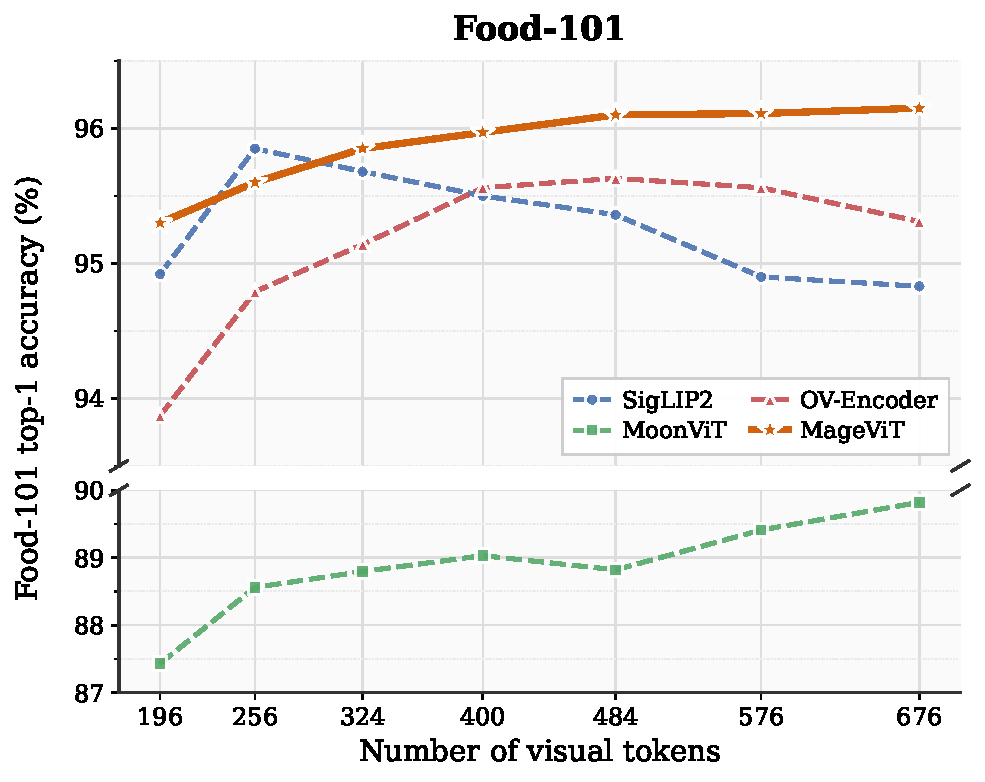
\includegraphics[width=0.49\linewidth]
    {figures/ViT_food101.pdf}
    \hfill
    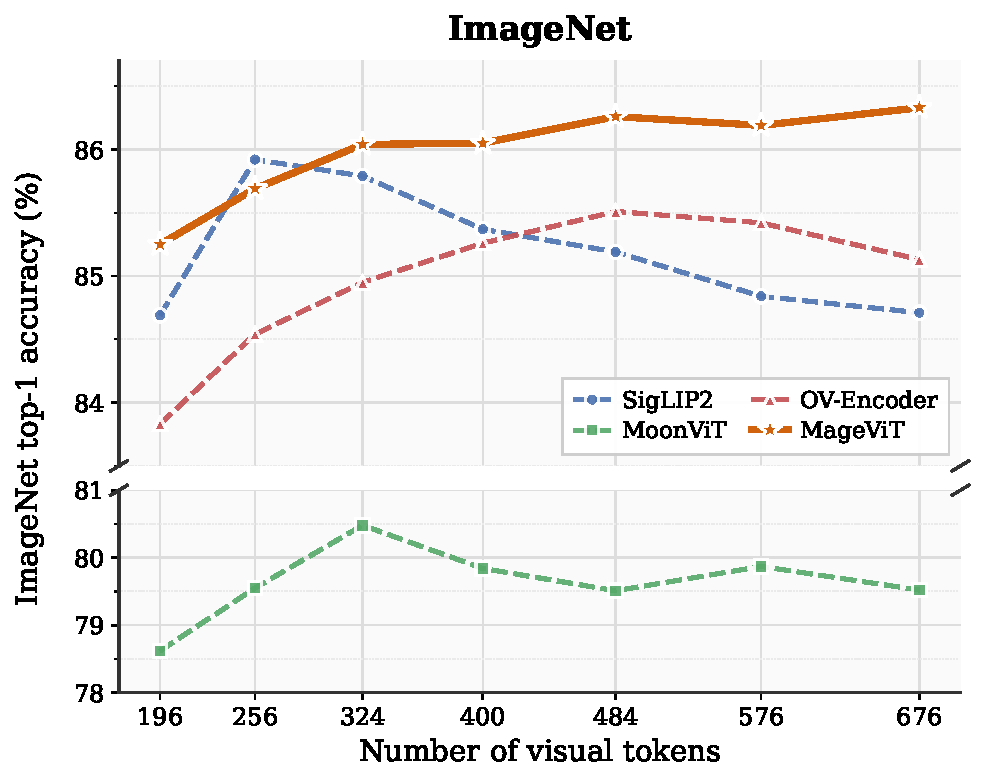
\includegraphics[width=0.49\linewidth]
    {figures/ViT_imagenet.pdf}
    \caption{
    \textbf{Effect of the visual-token budget on image representation
    quality.} We evaluate frozen visual features on Food-101 and ImageNet while increasing the number of input visual tokens. \magevit, which is trained with variable-resolution inputs, consistently benefits from larger token budgets and achieves its best performance at the highest evaluated resolution. In contrast, the fixed-resolution baselines generally saturate or degrade after reaching their optimal token budget.
    }
    \label{fig:vit_variable_resolution}
\end{figure*}



    
\subsection{Evaluation of Mage-ViT}
\label{sec:magevit_eval}
We evaluate \magevit from three perspectives: representation quality under limited pre-training data, the effect of native-resolution training across visual-token budgets, and robustness to different codec families. Image representations are evaluated using linear probes, while video representations are evaluated using attentive probes. Unless otherwise specified, all visual encoders remain frozen.



\begin{table}[t]
\centering
\small
\setlength{\tabcolsep}{6pt}
\definecolor{canvascol}{gray}{0.45}
\newcommand{\cv}[1]{{\color{canvascol}#1}}
\caption{
\textbf{Cross-codec robustness of codec-guided patch selection.}
We compare the HEVC selector used during training with the neural
codec DCVC-RT at inference time, without codec-specific retraining.
We report the task score and the average token \cv{Canvas} per video.
DCVC-RT is constrained to use no more tokens than HEVC.}
%\textbf{Robustness of codec-based patch selection across video understanding, temporal grounding, and spatial reasoning benchmarks.} We report the benchmark \emph{Score} and the average token \cv{Canvas} per video for the traditional codec (HEVC) and the neural codec (DCVC-RT), at a matched token budget (Canvas $\le$ HEVC).}
\label{tab:dcvc_vs_hevc}
\begin{adjustbox}{max width=\textwidth}
\begin{tabular}{l c c c c}
\toprule
& \multicolumn{2}{c}{Traditional: HEVC~\cite{sullivan2012hevc}} & \multicolumn{2}{c}{Neural: DCVC-RT~\cite{jia2025towards}} \\
\cmidrule(lr){2-3} \cmidrule(lr){4-5}
Benchmark & Score & \cv{Canvas} & Score & \cv{Canvas} \\
\midrule
\multicolumn{5}{l}{\textit{Video QA}} \\
MV-Bench~\cite{bench_mvbench}             & 65.1 & \cv{34.0} & 66.5 & \cv{30.5} \\
NextQA~\cite{bench_nextqa}               & 83.1 & \cv{32.7} & 82.6 & \cv{32.1} \\
TempCompass~\cite{bench_tempcompass}          & 62.3 & \cv{34.0} & 61.7 & \cv{31.1} \\
VideoMME~\cite{bench_videomme}             & 64.0 & \cv{33.2} & 64.3 & \cv{30.2} \\
LongVideoBench~\cite{bench_longvideobench}       & 61.3 & \cv{32.6} & 60.0 & \cv{29.3} \\
LVBench~\cite{bench_lvbench}              & 41.8 & \cv{32.2} & 43.5 & \cv{29.6} \\
MLVU-dev~\cite{bench_mlvu}             & 68.7 & \cv{33.6} & 66.1 & \cv{29.9} \\
\midrule
\multicolumn{5}{l}{\textit{Temporal grounding}} \\
Charades~\cite{bench_charades_sta}             & 31.4 & \cv{33.7} & 31.6 & \cv{32.0} \\
Timelens-Charades~\cite{zhang2025timelens}    & 50.7 & \cv{33.5} & 50.5 & \cv{31.9} \\
Timelens-ActivityNet~\cite{zhang2025timelens} & 45.4 & \cv{33.7} & 44.2 & \cv{31.4} \\
Timelens-QVHighlight~\cite{zhang2025timelens} & 57.4 & \cv{34.3} & 57.5 & \cv{30.7} \\
\midrule
\multicolumn{5}{l}{\textit{Spatial reasoning}} \\
VSI-Bench~\cite{yang2024vsi}            & 64.3 & \cv{32.8} & 63.7 & \cv{31.3} \\
\midrule
\textbf{Avg}         & \textbf{58.0} & \cv{\textbf{33.4 (100\%)}} & \textbf{57.7} & \cv{\textbf{30.8 (92\%)}} \\
\bottomrule
\end{tabular}
\end{adjustbox}
\end{table}


\subsubsection{Learning Strong Visual Representations from Limited Data}
\label{sec:magevit_data_efficiency}

As summarized in \cref{tab:summary_img_video}, we comprehensively evaluate \magevit on both standard image recognition benchmarks via linear probing and video action/event recognition via attentive probing. Across both modalities, \magevit demonstrates strong representation capacities without requiring massive web-scale pre-training datasets.


\paragraph{Image representation performance.}
On standard 2D image benchmarks, \magevit delivers performance that consistently rivals or exceeds top-tier visual encoders trained on billions of images. Specifically, \magevit achieves the highest top-1 accuracy on CIFAR-10 (\textbf{99.33\%}) and exhibits highly competitive performance on coarse-grained and fine-grained classification tasks, such as SUN397 (\textbf{82.01\%}), Food-101 (\textbf{95.60\%}), and ImageNet-1K (\textbf{85.69\%}). Notably, its performance closely matches SigLIP2 (\textbf{85.92\%} on ImageNet) and surpasses established strong backbones including MetaCLIP2, AIMv2, and OV-Encoder. Importantly, while OV-Encoder relies on a smaller $14\times14$ patch size, \magevit adopts a larger $16\times16$ patch grid, achieving comparable or superior representation quality with fewer visual tokens. This confirms that our pre-training scheme effectively constructs a highly transferable and semantically rich feature space for static visual concepts using significantly fewer visual tokens and pre-training samples.

\paragraph{Video representation performance and temporal adaptation.}
When extended to temporal video understanding, \magevit demonstrates superior temporal modeling and efficiency, particularly in motion-heavy and long-horizon scenarios:
\begin{itemize}[leftmargin=*]
    \item \textbf{Chunk-wise Evaluation:} Under the standard 16-frame uniform sampling protocol, \magevit achieves a top-1 accuracy of \textbf{85.13\%} on HMDB-51 and \textbf{84.83\%} on Kinetics-400 (K400), outperforming strong baselines such as SigLIP (\textbf{78.80\%} and \textbf{79.10\%}) and DINOv3 (\textbf{79.70\%} and \textbf{83.90\%}). On fine-grained action perception benchmarks like Diving-48 (\textbf{60.45\%}), \magevit significantly outperforms traditional image-centric models, highlighting its robust spatial-temporal feature extraction.
    \item \textbf{Codec-based Sparse Sampling:} When leveraging sparse patch selection across an expanded temporal context of 64 frames under the exact same visual token budget (4096 tokens), \magevit exhibits substantial performance boosts on motion-critical tasks. Specifically, the accuracy on Diving-48 jumps from \textbf{60.45\%} to \textbf{64.14\%} (+3.69\%), and HMDB-51 reaches a peak accuracy of \textbf{85.17\%}. This confirms that the spatio-temporal representations learned by \magevit naturally pair with codec-driven sparse tokenization, enabling the model to capture fine-grained temporal dynamics over longer video horizons without increasing computational or memory overhead.
\end{itemize}


\begin{promptbox}
\large
\textbf{\textit{Finding 1:}}
\textbf{Web-Scale Pre-training is Not Essential for VLM Visual Encoders.}
Despite being trained from scratch on a modest corpus, \magevit achieves visual representation quality competitive with flagship encoders like SigLIP2, proving that architectural and objective design can effectively substitute for web-scale pre-training data.
\end{promptbox}



\subsubsection{Native-Resolution Scaling across Visual-Token Budgets}
\label{sec:magevit_token_scaling}



To further evaluate how visual representations adapt to flexible input resolutions, we analyze performance across an increasing visual token budget (from 196 to 676 tokens per image) on Food-101 and ImageNet-1K, as shown in Fig.~\ref{fig:vit_variable_resolution}.

\paragraph{Monotonic resolution scaling vs. fixed-resolution degradation.}
Visual encoders exhibit fundamentally distinct scaling behaviors depending on their pre-training resolution strategies:
\begin{itemize}[leftmargin=*]
    \item \textbf{Fixed-Resolution Baselines (SigLIP2 \& OV-Encoder):} Because these models are pre-trained on fixed spatial grids, evaluating them under larger token budgets introduces severe positional distribution shifts. Consequently, SigLIP2 reaches its peak performance at 256 tokens on ImageNet ($\sim 85.9\%$) and continuously degrades as the token budget expands to 676 ($\sim 84.7\%$). Similarly, OV-Encoder experiences a clear performance drop beyond 484 tokens.
    \item \textbf{Variable-Resolution Encoders (MoonViT \& \magevit):} Encoders pre-trained with variable-resolution objectives naturally adapt to flexible spatial formats. While MoonViT avoids high-resolution collapse, its overall representation capacity remains low across all budget settings. In contrast, \magevit achieves the best of both worlds: its representation quality monotonically improves as the visual token budget increases—reaching peak accuracy at 676 tokens ($>96.1\%$ on Food-101 and $>86.3\%$ on ImageNet)—while consistently outperforming all baselines at every evaluated resolution.
\end{itemize}
This superior extrapolation capacity confirms that \magevit seamlessly accommodates dynamic visual sequence lengths, making it an ideal visual backbone for Large Multimodal Models (LMMs).

\begin{promptbox}
\large
\textbf{\textit{Finding 2:}}
\textbf{Variable-Resolution Pre-training Enables Continuous Monotonic Scaling with Resolution and Token Budgets.}
While fixed-resolution vision encoders suffer from sharp performance degradation when evaluated at higher resolution budgets, \magevit leverages variable-resolution pre-training to achieve continuous, monotonic quality gains without saturation.
\end{promptbox}


\begin{table*}[t]
\centering
\scriptsize
\setlength{\tabcolsep}{4pt}
\caption{\textbf{Image understanding and spatial intelligence} across STEM/math, document understanding, general VQA, perception/alignment, and 2D/3D scene geometry, embodied/viewpoint, cross-view, and relational spatial benchmarks. \colorbox{bestblue}{Dark blue} and \colorbox{secondblue}{light blue} background colors indicate the best and second-best results per row, respectively.}
\label{tab:understand_image}
\begin{adjustbox}{max width=\textwidth, max totalheight=0.9\textheight}
\begin{tabular}{l c c c c}
\toprule
Benchmark & \magevl-4B & Qwen3-VL-4B~\cite{qwen3vl} & Phi-4-MM-5.6B ~\cite{abdin2024phi4} & Phi-4-R-V-15B~\cite{aneja2026phi4reasoningvision15btechnicalreport} \\
\midrule
\multicolumn{5}{l}{\textit{Document understanding}} \\
DocVQA-val~\cite{bench_docvqa}         & \best{95.14}   & \second{94.69} & 92.79          & 76.20 \\
InfoVQA-val~\cite{bench_infographicvqa}& \best{80.33}   & \second{79.50} & 71.84          & 55.41 \\
AI2D w/ Mask~\cite{bench_ai2d}         & \best{83.16}   & 81.54          & 81.83          & \second{82.87} \\
AI2D w/o Mask~\cite{bench_ai2d}                          & 91.87          & \second{92.20} & 91.35          & \best{93.81} \\
ChartQA~\cite{bench_chartqa}           & \best{84.88}   & \second{83.96} & 83.76          & 83.40 \\
OCRBench~\cite{bench_ocrbench}         & \best{81.80}   & 81.60          & \second{81.70} & 73.90 \\
CC-OCR Doc~\cite{bench_cc_ocr}         & \second{32.25} & \best{39.69}   & 4.99           & 17.65 \\
MultiDocVQA-val~\cite{bench_mp_docvqa}  & \best{87.46}   & \second{87.21} & 46.84          & 58.35 \\
DUDE~\cite{bench_dude}                 & \second{46.44} & \best{50.98}   & 3.78           & 34.34 \\
WebSRC-val~\cite{bench_websrc}         & \second{92.80} & \best{95.40}   & 71.30          & 76.60 \\
ChartQAPro~\cite{bench_chartqapro}     & \best{32.57}   & \second{26.79} & 0.13           & 25.38 \\
TextVQA-val~\cite{bench_textvqa}       & \second{77.28} & \best{80.55}   & 39.93          & 76.06 \\
CharXiv-Description~\cite{bench_charxiv}    & \second{75.85} & 74.40          & 18.65          & \best{75.98} \\
CharXiv-Reason~\cite{bench_charxiv}                         & \second{35.20} & 26.10          & 0.10           & \best{36.10} \\
\midrule
\multicolumn{5}{l}{\textit{General VQA}} \\
MMBench-EN-dev~\cite{bench_mmbench}   & \second{84.02} & 83.25          & 65.81          & \best{84.19} \\
MMBench-CN-dev~\cite{bench_mmbench}                         & \best{82.04}   & \second{80.58} & 75.17          & 79.47 \\
RealWorldQA~\cite{bench_realworldqa}   & 70.46          & \best{70.85}   & 60.65          & \second{70.72} \\
MMStar~\cite{bench_mmstar}             & \best{67.32}   & \second{62.04} & 61.24          & 59.63 \\
MME-Perception~\cite{bench_mme}        & \best{1709.54} & \second{1703.50}& 1409.66       & 1590.21 \\
SeedBench (All)~\cite{bench_seedbench} & \best{76.78}   & \second{75.65} & 68.28          & 73.70 \\
SeedBench-Image~\cite{bench_seedbench}                        & \best{79.32}   & \second{78.87} & 74.48          & 77.97 \\
SeedBench2-Plus~\cite{bench_seedbench2plus}& \second{69.21}& \best{69.65}   & 68.38          & 69.48 \\
MMT-val~\cite{bench_mmtbench}          & 64.47          & \best{66.52}   & 59.19          & \second{64.89} \\
CV-Bench~\cite{cambrian}               & \best{87.79}   & \second{85.37} & 57.09          & 81.31 \\
MME-RealWorld~\cite{bench_mmerealworld}& \best{66.52}   & \second{63.20} & 32.45          & 57.80 \\
MME-RealWorld-CN~\cite{bench_mmerealworld}                       & \second{61.33} & \best{63.09}   & 21.19          & 46.07 \\
\midrule
\multicolumn{5}{l}{\textit{Spatial intelligence}} \\
CV-Bench-2D~\cite{tong2024cambrian}                            & \best{82.13}   & \second{81.00} & 56.12          & 80.11 \\
CV-Bench-3D~\cite{tong2024cambrian}                            & \best{94.75}   & \second{92.30} & 56.92          & 82.50 \\
BLINK~\cite{bench_blink}               & \best{65.11}   & \second{65.10} & 35.24          & 57.80 \\
EmbSpatial~\cite{bench_embspatial}     & \best{82.67}   & \second{77.50} & 41.51          & 72.67 \\
CRPE-Relation~\cite{bench_crpe}        & \second{76.12} & \best{77.70}   & 34.60          & 74.46 \\
CrossPoint~\cite{wang2025crosspoint}                             & \best{80.00}   & 26.90          & 12.20          & \second{47.73} \\
ERQA~\cite{bench_erqa}                 & 36.00          & \best{42.30}   & 30.75          & \second{40.25} \\
MMSI-Bench~\cite{bench_mmsibench}      & 28.20          & \best{31.00}   & \second{28.80} & 25.70 \\
SAT~\cite{bench_sat}                   & \second{67.33} & \best{69.30}   & 55.33          & 66.67 \\
\bottomrule
\end{tabular}
\end{adjustbox}
\end{table*}

\begin{table}[t]
\centering
\small
\setlength{\tabcolsep}{6pt}
\caption{\textbf{Video understanding and temporal grounding.} \magevl and Qwen3-VL-4B share the 4B Qwen3 LLM backbone and differ only in the visual front-end (Qwen3-VL: dense ViT; \magevl: \magevit); Phi-4-MM and Phi-4-R-V are reported for reference. \colorbox{bestblue}{Dark blue} and \colorbox{secondblue}{light blue} background colors indicate the best and second-best results per row, respectively.}
\label{tab:understand_video}
\begin{adjustbox}{max width=\textwidth}
\begin{tabular}{l c c c c}
\toprule
Benchmark & \magevl-4B & Qwen3-VL-4B~\cite{qwen3vl} & Phi-4-MM-5.6B ~\cite{abdin2024phi4} & Phi-4-R-V-15B~\cite{aneja2026phi4reasoningvision15btechnicalreport} \\
\midrule
\multicolumn{5}{l}{\textit{Video QA}} \\
MV-Bench~\cite{bench_mvbench}          & \second{65.1}  & \best{66.7}   & 44.9           & 49.2 \\
NextQA~\cite{bench_nextqa}            & \best{83.1}    & \second{79.8} & 54.1           & 69.0 \\
VideoMME~\cite{bench_videomme}        & \best{64.0}    & \second{59.7} & 44.7           & 55.3 \\
LongVideoBench~\cite{bench_longvideobench}& \best{61.3} & \second{57.7} & 41.14          & 51.2 \\
LVBench~\cite{bench_lvbench}          & \best{41.8}    & \second{39.2} & 25.31          & 34.4 \\
MLVU-dev~\cite{bench_mlvu}            & \best{68.7}    & \second{61.5} & 44.18          & 51.8 \\
VideoMME (w/ sub.)~\cite{bench_videomme}                    & \second{66.3}  & \best{70.2}   & 45.4           & 58.3 \\
VideoMME-V2~\cite{fu2026video}                           & \second{24.3}  & \best{24.4}   & 19.2           & 23.9 \\
VideoEval-Pro~\cite{bench_videoevalpro}& \best{45.2}   & \second{20.7} & 14.35          & 16.8 \\
JumpScore~\cite{llavaonevision2}                             & \best{45.60}   & \second{3.82} & 3.61           & 1.53 \\
MMOU-Test-Mini~\cite{goel2026mmou}                        & \second{39.3}  & 38.1          & 32.22          & \best{51.9} \\
\midrule
\multicolumn{5}{l}{\textit{Temporal grounding}} \\
Timelens-Charades~\cite{zhang2025timelens}                     & \best{50.7}    & \second{43.1} & 4.09           & 20.6 \\
Timelens-ActivityNet~\cite{zhang2025timelens}                  & \best{45.4}    & \second{28.4} & 2.03           & 23.0 \\
Timelens-QVHighlight~\cite{zhang2025timelens}                  & \best{57.4}    & \second{34.9} & 2.47           & 11.6 \\
\midrule
\multicolumn{5}{l}{\textit{Spatial reasoning}} \\
VSI-Bench~\cite{yang2024vsi}          & \best{64.3}    & \second{53.3} & 24.09          & 25.5 \\
\midrule
\multicolumn{5}{l}{\textit{Tracking (J\&F)}} \\
Ref-DAVIS17~\cite{bench_refdavis17}   & \best{25.83}   & \second{7.48} & 3.14           & 2.15 \\
MeViS-ValidU~\cite{bench_mevis}       & \best{22.55}   & 3.16          & \second{10.28} & 1.53 \\
ReasonVOS~\cite{bench_revos}          & \best{17.76}   & 9.66          & 9.50           & \second{9.77} \\
Ref-YT-VOS~\cite{bench_refytvos}      & \best{25.57}   & \second{5.28} & 8.64           & 3.85 \\
\bottomrule
\end{tabular}
\end{adjustbox}
\end{table}

\subsubsection{Robust Token Selection across Codec Families}
\label{sec:magevit_codec_robustness}




As introduced in \cref{sec:magevit_arch}, \magevit uses a codec-derived importance map to select informative patches from predicted frames. During training, this map is computed from HEVC~\citep{sullivan2012hevc} using motion-vector magnitude and residual energy. Since these signals are specific to the coding process of a traditional codec, an important question is whether the resulting token-selection strategy generalizes to fundamentally different codec families.

We evaluate this by replacing the HEVC-based selector at inference time with DCVC-RT~\citep{jia2025towards}, a neural video codec whose learned probability model estimates local coding cost through negative log-likelihood. No codec-specific retraining or adaptation is applied. As shown in \cref{tab:dcvc_vs_hevc}, the two selectors achieve nearly identical average performance across video QA, temporal grounding, and spatial reasoning benchmarks, while the neural-codec selector uses a smaller average token canvas. Performance also remains comparable across most individual tasks, with no consistent degradation after switching codec families.

These results indicate that codec-guided token selection does not depend on the particular motion-estimation, residual-coding, or probability model used by a codec. Although HEVC and DCVC-RT implement compression through different mechanisms, both assign greater coding cost to regions that are difficult to predict from temporal context. Motion-vector magnitude, residual energy, and neural-codec negative log-likelihood therefore provide different estimates of the same underlying signal: local temporal predictability.

Importantly, \magevit consumes only the resulting patch-importance map, rather than codec-specific syntax or latent representations. The visual tokenizer is therefore decoupled from the mechanism used to estimate coding difficulty. This establishes temporal predictability as a transferable criterion for allocating visual tokens and allows codec-guided tokenization to generalize across traditional and neural compression systems.


\subsection{Evaluation of Mage-VL}
\label{sec:image_video_eval}
\subsubsection{Image Understanding}


\Cref{tab:understand_image} reports model performance across three core capability dimensions: document understanding, which aligns with Microsoft's primary domain applications; general VQA, which evaluates general multimodal proficiency; and spatial intelligence, which represents a core strategic focus of \magevl.
Against the matched-LLM Qwen3-VL-4B control, \magevl is competitive on aggregate and clearly ahead on the categories that our caption-heavy curriculum targets. On document, OCR, and chart understanding, \magevl leads on the majority of benchmarks---including DocVQA ($95.14$), InfoVQA ($80.33$), ChartQA ($84.88$), OCRBench ($81.80$), and AI2D-with-mask ($83.16$)---consistent with the dense-recaptioning and verbatim-OCR emphasis of our data pipeline. On general VQA, the two models trade wins within small margins, with \magevl achieving top results on MMStar ($67.32$), MME-Perception ($1709.54$), and CV-Bench ($87.79$), while comprehensively surpassing the similarly-sized Phi-4-MM across the board. The clearest and most consistent gains appear in the spatial-intelligence block: \magevl improves over Qwen3-VL on CV-Bench-3D ($94.75$ vs.\ $92.30$), EmbSpatial ($82.67$ vs.\ $77.50$), and dramatically on cross-view point correspondence (CrossPoint $80.00$ vs.\ $26.90$), where codec-aligned patchification preserves the dense, geometrically-consistent structure that viewpoint matching requires. Despite using roughly a quarter of its parameters, \magevl also surpasses Phi-4-R-V (15B) on the large majority of these spatial benchmarks. 

\subsubsection{Video Understanding}


\Cref{tab:understand_video} reports video understanding under the same matched-LLM comparison, so that \magevl and Qwen3-VL-4B differ only in the visual front-end.
\magevl improves on most video-QA benchmarks, including VideoMME ($+4.3$), MLVU ($+7.2$), LongVideoBench ($+3.5$), LVBench ($+2.6$), NextQA ($+3.3$), and especially the long and realistic VideoEval-Pro ($+24.5$). Qwen3-VL remains stronger on MV-Bench, TempCompass, and MMVU, which lean more on dense per-frame appearance than on temporal localization. The gains concentrate in \emph{localization-heavy} regimes: on temporal grounding \magevl improves by $+7.6$, $+17.1$, and $+22.5$ on the Timelens Charades/ActivityNet/QVHighlight splits; on video spatial reasoning by $+11.0$ on VSI-Bench; and on referring-video tracking by roughly $+18$ to $+20$ J\&F points on Ref-DAVIS17, MeViS, and Ref-YouTube-VOS (and $+8.1$ on ReasonVOS).
 
Notably, these competitive long VideoQA capabilities are achieved \emph{without any} long VideoQA SFT; instead, \magevl relies solely on short video SFT alongside detailed video captions. The dense temporal-visual alignment established by video captions enables the base LLM to handle VideoQA tasks zero-shot, bypassing the need for heavy VideoQA instruction tuning. \Cref{tab:understand_video_tc8} further shows that the lightweight tc8 setting preserves most of these gains at a fraction of the visual-token cost, confirming that the advantage does not hinge on a large frame budget.

% Importantly, the training mixture includes short-video QA supervision but no dedicated long-video QA data. Long-video capabilities are instead learned primarily from temporally detailed captions and codec-native long-context training. The strong results on LongVideoBench, LVBench, MLVU-dev, VideoMME, and VideoEval-Pro therefore indicate that short-video instruction tuning can transfer to substantially longer contexts when combined with fine-grained long-video caption supervision. \Cref{tab:understand_video_tc8} further shows that the lower-budget tc8 and tc16 settings retain competitive performance, demonstrating that these capabilities do not depend exclusively on the largest visual budget.

\begin{promptbox}
\large
\textbf{\textit{Finding 3:}}
\textbf{Dense Video Captions Bypass Long VideoQA SFT.}
Without explicit long VideoQA instruction tuning, fine-tuning solely on video detailed captions (alongside short video SFT) is sufficient for strong VideoQA capabilities. High-quality captioning establishes solid temporal-visual alignment, allowing the base LLM to generalize to long VideoQA zero-shot.
\end{promptbox}



\begin{table*}[t]
\centering
\scriptsize
\setlength{\tabcolsep}{3.5pt}
\caption{\textbf{Video performance and evaluation efficiency across token/codec budgets.}
Performance uses each benchmark's primary metric ($\uparrow$); evaluation efficiency is reported as wall-clock Time in seconds ($\downarrow$) on a single 8$\times$B200 node. Qwen3-VL and Phi-4-R-V use 32 frames, and their time excludes estimated video-loading time ($1.01N/8$ and $1.01N$ for $N$ samples, respectively), whereas Mage-VL reports full measured wall-clock time. \colorbox{bestblue}{Dark blue} and \colorbox{secondblue}{light blue} backgrounds indicate the best and second-best performance per row.}
\label{tab:understand_video_tc8}
\begin{adjustbox}{max width=\textwidth}
\begin{tabular}{l *{5}{c c}}
\toprule
& \multicolumn{2}{c}{\magevl-4B (tc8)} 
& \multicolumn{2}{c}{\magevl-4B (tc16)} 
& \multicolumn{2}{c}{\magevl-4B (tc32)} 
& \multicolumn{2}{c}{Qwen3-VL-4B~\cite{qwen3vl}} 
& \multicolumn{2}{c}{Phi-4-R-V-15B~\cite{aneja2026phi4reasoningvision15btechnicalreport}} \\
\cmidrule(lr){2-3} \cmidrule(lr){4-5} \cmidrule(lr){6-7} \cmidrule(lr){8-9} \cmidrule(lr){10-11}
Benchmark & Perf. ($\uparrow$) & Time (s) ($\downarrow$) & Perf. ($\uparrow$) & Time (s) ($\downarrow$) & Perf. ($\uparrow$) & Time (s) ($\downarrow$) & Perf. ($\uparrow$) & Time (s) ($\downarrow$) & Perf. ($\uparrow$) & Time (s) ($\downarrow$) \\
\midrule
\multicolumn{11}{l}{\textit{Video QA}} \\
MV-Bench~\cite{bench_mvbench}             & 65.1 & 893 & \second{65.5} & 972  & 65.1          & 1054 & \best{66.7}   & 1268 & 49.2 & 2923 \\
NextQA~\cite{bench_nextqa}               & 80.8 & 415 & \second{82.4} & 502  & \best{83.1}   & 642  & 79.8          & 1460 & 69.0 & 29024 \\
TempCompass~\cite{bench_tempcompass} & 61.5 & 389 & \second{62.4} & 510 & 62.3 & 729  & \best{72.7}   & 433  & 34.8 & 3518 \\
VideoMME~\cite{bench_videomme}             & 57.9 & 270 & \second{61.8} & 439  & \best{64.0}   & 534  & 59.7          & 463  & 55.3 & 3187 \\
LongVideoBench~\cite{bench_longvideobench}       & 56.2 & 279 & \best{63.1}   & 1308 & \second{61.3} & 345  & 57.7          & 365  & 51.2 & 2617 \\
LVBench~\cite{bench_lvbench}              & 38.9 & 213 & 38.9          & 266  & \best{41.8}   & 333  & \second{39.2} & 554  & 34.4 & 2692 \\
MLVU-dev~\cite{bench_mlvu}             & 63.2 & 296 & \second{65.6} & 326  & \best{68.7}   & 361  & 61.5          & 786  & 51.8 & 6326 \\
\midrule
\multicolumn{11}{l}{\textit{Temporal grounding}} \\
Charades~\cite{bench_charades_sta} & 34.1 & 534 & 33.2 & 417 & 31.4 & 729 & \best{45.9} & 707 & 0.3 & 1844 \\
Timelens-Charades~\cite{zhang2025timelens}    & 46.4 & 483 & \second{50.4} & 538  & \best{50.7}   & 623  & 43.1          & 643  & 20.6 & 3607 \\
Timelens-ActivityNet~\cite{zhang2025timelens} & 32.9 & 554 & \second{39.7} & 622  & \best{45.4}   & 785  & 28.4          & 766  & 23.0 & 4611 \\
Timelens-QVHighlight~\cite{zhang2025timelens} & 42.6 & 357 & \second{52.1} & 358  & \best{57.4}   & 421  & 34.9          & 402  & 11.6 & 1643 \\
\midrule
\multicolumn{11}{l}{\textit{Spatial reasoning}} \\
VSI-Bench~\cite{yang2024vsi}            & 55.7 & 329 & \second{61.1} & 368  & \best{64.3}   & 537  & 53.3          & 255  & 25.5 & 4360 \\
\bottomrule
\end{tabular}
\end{adjustbox}
\end{table*}


Beyond temporal grounding and video-level reasoning, we observe an intriguing positive transfer from dynamic video training to static spatial intelligence. 
While traditional paradigms often treat spatial reasoning and temporal video understanding as isolated capabilities, exposure to continuous video streams—rich in egocentric perspective shifts, camera trajectories, and object-environment interactions—provides a strong inductive bias for fine-grained 2D/3D geometric perception. 
Although rigorous single-variable ablations remain challenging due to the tightly coupled joint pre-training recipe, our empirical results across spatial benchmarks (e.g., CV-Bench and EmbSpatial) strongly support this cross-task synergy.

\begin{promptbox}
\large
\textbf{\textit{Finding 4:}}
\textbf{Dynamic Video Training Synergizes with Spatial Intelligence.}
Incorporating dynamic video sequences with rich viewpoint transitions and spatial interactions enhances 2D/3D spatial reasoning capabilities, allowing \magevl to achieve strong performance on static spatial benchmarks alongside temporal video tasks.
\end{promptbox}


\subsection{Streaming Video Understanding}
\label{sec:streaming_video_understanding}

To systematically evaluate \magevl in continuous video streams, we investigate both its \emph{response timing} (when to speak) and \emph{response quality} (what to say), accompanied by a qualitative case study on real-world sports broadcasts.

% ------------------ 1. Response Timing ------------------
\paragraph{Response timing.} 
We evaluate our codec-native streaming model on the SoccerNet-Caption validation split following the StreamMind evaluation protocol~\citep{ding2025streammindunlockingframerate}. The decision gate is evaluated at every valid streaming position via an $\mathrm{argmax}$ over the \emph{silent}/\emph{speak} logits using exact canvas-position matching with zero temporal tolerance. 
We report TriggerAcc (fraction of correctly predicted gate positions) and TimVal (which balances speak and silence correctness), both macro-averaged across 98 match halves. Additionally, raw per-position F1, ROC-AUC, and PR-AUC are reported without temporal tolerance. 

For reference, baseline numbers for StreamMind are directly taken from its original publication~\citep{ding2025streammindunlockingframerate}. Notably, StreamMind was explicitly trained in-distribution on SoccerNet-Caption, whereas \magevl achieves superior event-triggering performance under strict, zero-tolerance canvas-position matching without domain-specific over-tuning. Note that JoyAI is evaluated at 1~Hz with a relaxed $\pm1$-second window.

As presented in Table~\ref{tab:response_timing}, JoyAI-VL-Interaction exhibits a severe bias toward predicting silence. Due to the extreme class imbalance in SoccerNet-Caption (where silent frames dominate), JoyAI achieves an artificially inflated TriggerAcc ($97.98\%$) but suffers a severe degradation on precision-sensitive and balanced metrics (e.g., $19.25\%$ TimVal and $3.55\%$ F1). 
In contrast, \magevl significantly outperforms StreamMind—despite StreamMind being trained \emph{in-distribution} on SoccerNet-Caption—achieving $79.21\%$ TriggerAcc and a state-of-the-art $55.54\%$ TimVal. This superior performance across ROC-AUC ($83.14\%$) and PR-AUC ($9.30\%$) demonstrates that \magevl achieves well-calibrated, timely response triggering without collapsing into trivial silent predictions.

\begin{table}[t]
\centering
\small
\setlength{\tabcolsep}{6pt}
\caption{\textbf{Response timing evaluation on SoccerNet-Caption~\cite{mkhallati2023soccernet}.} Metrics include TriggerAcc, TimVal, per-position F1, ROC-AUC, and PR-AUC. Best results per column are in \textbf{bold}.}
\label{tab:response_timing}
\begin{tabular}{l c c c c c}
\toprule
Method & TriggerAcc & TimVal & F1 & ROC-AUC & PR-AUC \\
\midrule
StreamMind~\cite{ding2025streammindunlockingframerate} & 52.18 & 47.36 & -- & -- & -- \\
JoyAI-VL-Interaction-9B~\cite{joyai2026vlinteraction}     & \textbf{97.98} & 19.25 & 3.55 & 56.26 & 1.68 \\
Mage-VL-4B                                      & 79.21 & \textbf{55.54} & \textbf{16.35} & \textbf{83.14} & \textbf{9.30} \\
\bottomrule
\end{tabular}
\end{table}


% ------------------ 2. Response Quality ------------------
\paragraph{Response quality.} 
Beyond timing accuracy, we evaluate the streaming perception quality of \magevl on OVO-Bench~\citep{li2025ovobench} under the recent-window protocol established by SimpleStream~\citep{shen2026simplestream}, where queries are answered using the four most recent frames sampled at 1\,fps. 
As detailed in Table~\ref{tab:main_ovo}, \magevl achieves $79.84\%$ average accuracy on Real-Time Visual Perception and $48.15\%$ on Backward Tracing, establishing a new state-of-the-art overall OVO-Bench score of $64.00\%$ among streaming architectures. Crucially, this competitive real-time perception capability is attained without requiring streaming-specific fine-tuning or heavy external memory modules.

\begin{table*}[t]
\centering
\caption{\textbf{Results on OVO-Bench.}
Baseline results and table structure are adapted from SimpleStream~\citep{shen2026simplestream}.
OVO-Bench reports per-task accuracy under Real-Time Visual Perception and Backward Tracing.
$\dagger$: Qwen2.5-VL-7B + HERMES (4K tokens).
OCR, ACR, ATR, STU, FPD, and OJR denote Optical Character Recognition, Action Recognition,
Attribute Recognition, Spatial Understanding, Future Prediction, and Object Recognition;
EPM, ASI, and HLD denote Episodic Memory, Action Sequence Identification, and Hallucination
Detection. ``Avg.'' is the mean of the Real-Time and Backward category averages. 
\colorbox{bestblue}{Dark blue} and \colorbox{secondblue}{light blue} backgrounds highlight the best and second-best results across all models, respectively.}
\label{tab:main_ovo}
\renewcommand{\arraystretch}{1.08}
\setlength{\tabcolsep}{3pt}
\resizebox{\textwidth}{!}{%
\begin{tabular}{lc|cccccc|c|ccc|c|c}
\toprule
\multirow{3}{*}{Model} & \multirow{3}{*}{\#Frames}
& \multicolumn{12}{c}{\textit{OVO-Bench}~\citep{li2025ovobench}} \\
\cmidrule(lr){3-14}
& & \multicolumn{7}{c|}{\textit{Real-Time Visual Perception}}
& \multicolumn{4}{c|}{\textit{Backward Tracing}}
& \multirow{2}{*}{Avg.} \\
\cmidrule(lr){3-9} \cmidrule(lr){10-13}
& & OCR & ACR & ATR & STU & FPD & OJR & Avg.
& EPM & ASI & HLD & Avg. & \\
\midrule
Human & --
& 94.0 & 92.6 & 94.8 & 92.7 & 91.1 & 94.0 & 93.2
& 92.6 & 93.0 & 91.4 & 92.3 & 92.77 \\
\midrule
\multicolumn{14}{c}{\textit{Offline Video LLMs}} \\
\midrule
Qwen2.5-VL-7B~\cite{bai2025qwen25vl} & 1\,fps
& 67.8 & 55.1 & 67.2 & 42.1 & 66.3 & 60.9 & 59.9
& 51.5 & 58.8 & 23.7 & 44.7 & 52.28 \\
LLaVA-Video-7B~\cite{model_llavavideo} & 64
& 69.1 & 58.7 & 68.8 & 49.4 & 74.3 & 59.8 & 63.5
& 56.2 & 57.4 & 7.5 & 40.4 & 51.95 \\
Qwen3-VL-4B~\cite{qwen3vl} & 64
& 77.9 & \second{69.7} & \second{77.6} & \second{60.1} & 76.2 & \best{75.5} & \second{72.8}
& \best{63.0} & \second{66.2} & 30.1 & \best{53.1} & \second{63.00} \\
\midrule
\multicolumn{14}{c}{\textit{Online / Streaming Video LLMs}} \\
\midrule
VideoLLM-online-8B~\cite{chen2024videollmonline} & 2\,fps
& 8.1 & 23.9 & 12.1 & 14.0 & 45.5 & 21.2 & 20.8
& 22.2 & 18.8 & 12.2 & 17.7 & 19.26 \\
Flash-VStream-7B~\cite{zhang2024flashvstream} & 1\,fps
& 24.2 & 29.4 & 28.5 & 33.7 & 25.7 & 28.8 & 28.4
& 39.1 & 37.2 & 5.9 & 27.4 & 27.90 \\
Dispider-7B~\cite{qian2025dispider} & 1\,fps
& 57.7 & 49.5 & 62.1 & 44.9 & 61.4 & 51.6 & 54.6
& 48.5 & 55.4 & 4.3 & 36.1 & 45.35 \\
TimeChat-Online-7B~\cite{model_timechatonline} & 1\,fps
& 75.2 & 46.8 & 70.7 & 47.8 & 69.3 & 61.4 & 61.9
& 55.9 & 59.5 & 9.7 & 41.7 & 51.80 \\
StreamForest-7B~\cite{model_streamforest} & 1\,fps
& 68.5 & 53.2 & 71.6 & 47.8 & 65.4 & 60.9 & 61.2
& \second{58.9} & 64.9 & 32.3 & 52.0 & 56.60 \\
Streamo-7B~\cite{model_streamo} & 1\,fps
& 79.2 & 57.8 & 75.0 & 49.4 & 64.4 & 70.1 & 66.0
& 54.6 & 52.0 & 31.7 & 46.1 & 56.05 \\
HERMES-7B$^\dagger$~\cite{model_hermes} & 1\,fps
& \second{85.2} & 64.2 & 71.6 & 53.4 & \second{74.3} & 65.2 & 69.0
& 48.5 & 62.2 & \best{37.6} & 49.4 & 59.20 \\
JoyAI-VL-Interaction-9B~\citep{joyai2026vlinteraction} & 1\,fps
& 72.5 & 61.5 & 75.0 & 59.0 & \best{78.2} & 64.1 & 68.4
& 62.0 & \best{70.9} & 12.9 & 48.6 & 58.50 \\
\textbf{\magevl-4B} & 1\,fps
& \best{94.63} & \best{83.49} & \best{79.31} & \best{74.16} & 70.30 & \second{77.17} & \best{79.84}
& 50.17 & 61.49 & \second{32.80} & \second{48.15} & \best{64.00} \\
\bottomrule
\end{tabular}%
}
\end{table*}


% ------------------ 3. Qualitative Illustration ------------------
\paragraph{Qualitative illustration.} 
Fig.~\ref{fig:streaming_case} presents a qualitative case study on a live 2026 World Cup broadcast between England and Argentina outside the SoccerNet evaluation split. As visualized, our codec front-end dynamically retains spatial patches ($16{\times}16$) associated with salient motion and novel visual details while suppressing temporally predictable background regions. Throughout routine gameplay ($02.16\text{s}$--$24.50\text{s}$), the event gate stays silent. At $29.36\text{s}$, upon detecting an active offensive play—where an England player drives toward the goal under close pursuit by an Argentina defender—the event gate triggers the language decoder to proactively generate a real-time commentary (\emph{``An England player drives toward goal, closely pursued by an Argentina defender as the attack develops.''}). This demonstrates the seamless synergy between codec-native sparse perception and event-driven response generation in demanding live streaming scenarios.

\begin{figure*}[h]
  \centering
  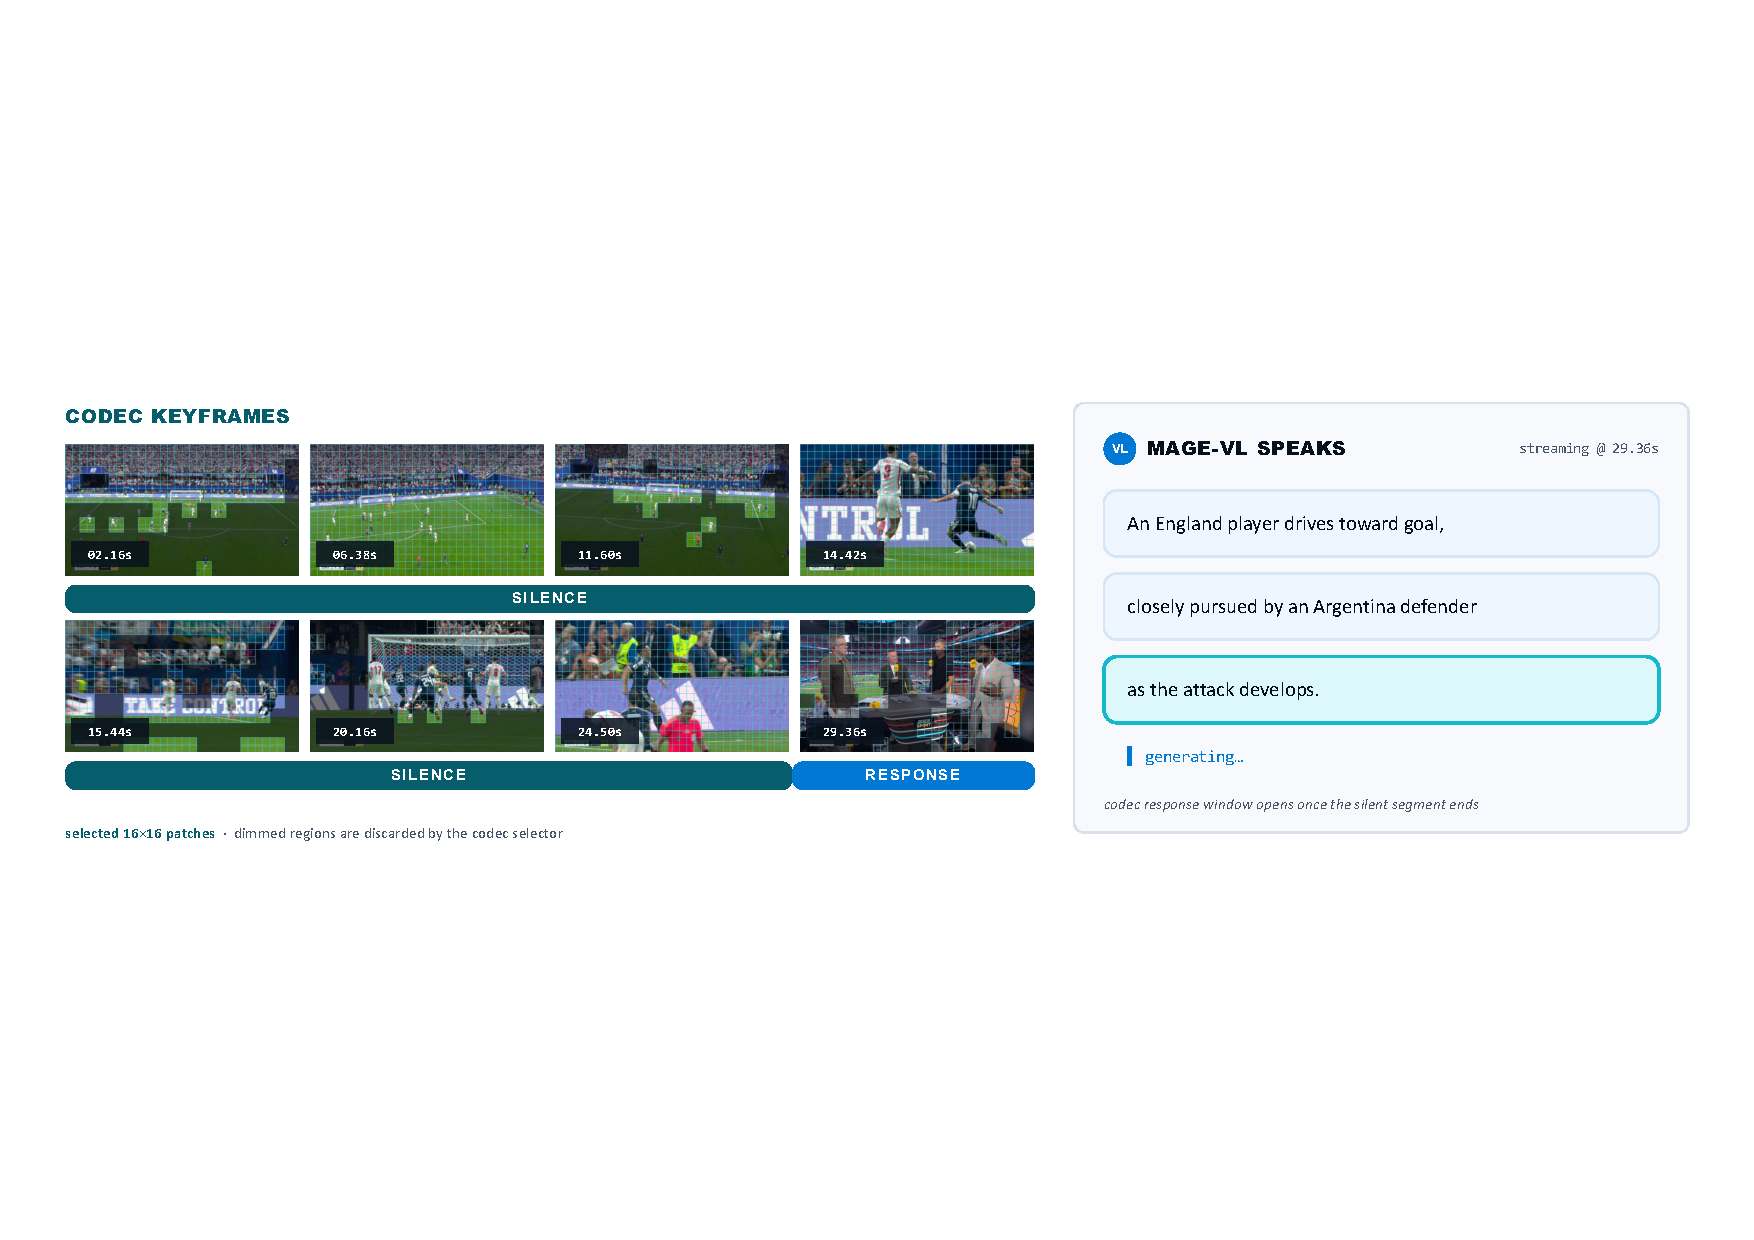
\includegraphics[width=\textwidth]{figures/streaming_case.pdf}
  \caption{\textbf{Codec-native proactive streaming on a 2026 World Cup broadcast (England vs. Argentina).}
  Eight frames from a causal match window visualize the $16{\times}16$ patches retained by the codec selector; dimmed regions are discarded as temporally predictable. The event gate remains silent through routine updates and triggers the language decoder at $29.36\text{s}$ when a response-worthy offensive play is observed. The speech bubble shows the real-time generated response.}
  \label{fig:streaming_case}
\end{figure*}





\subsection{Efficiency Analysis}
\label{sec:efficiency_analysis}

To understand how codec-native tokenization alters the trade-off between visual budget and downstream accuracy, we analyze both the scaling trends under matched visual input budgets and the wall-clock evaluation efficiency.

% ------------------ 1. Budget Formulation ------------------
\paragraph{Matched-budget setup.}
We evaluate \emph{codec-input efficiency} by comparing downstream performance under an equivalent nominal visual input capacity to the vision encoder. 
For the uniform baseline, \emph{frame-$N$} denotes Qwen3-VL-4B evaluated on $N \in \{4, 8, 16, 32, 64\}$ uniformly sampled RGB frames. For \magevl, \emph{tc-$N$} denotes a target budget of $N$ codec canvases, constructed via adaptive temporal grouping and salient patch packing over an $8\times$ denser source-frame sequence ($8N$ raw frames). Following LLaVA-OneVision-2~\cite{llavaonevision2}, both paradigms share identical vision architectures ($16{\times}16$ patch size, max 150K pixels per input canvas). Consequently, frame-$N$ and tc-$N$ subject the vision backbone to the same nominal token workload, but tc-$N$ adaptively concentrates representation capacity onto motion-salient regions across a significantly wider temporal horizon.

% ------------------ 2. Scaling Curves ------------------
\begin{figure*}[t]
  \centering
  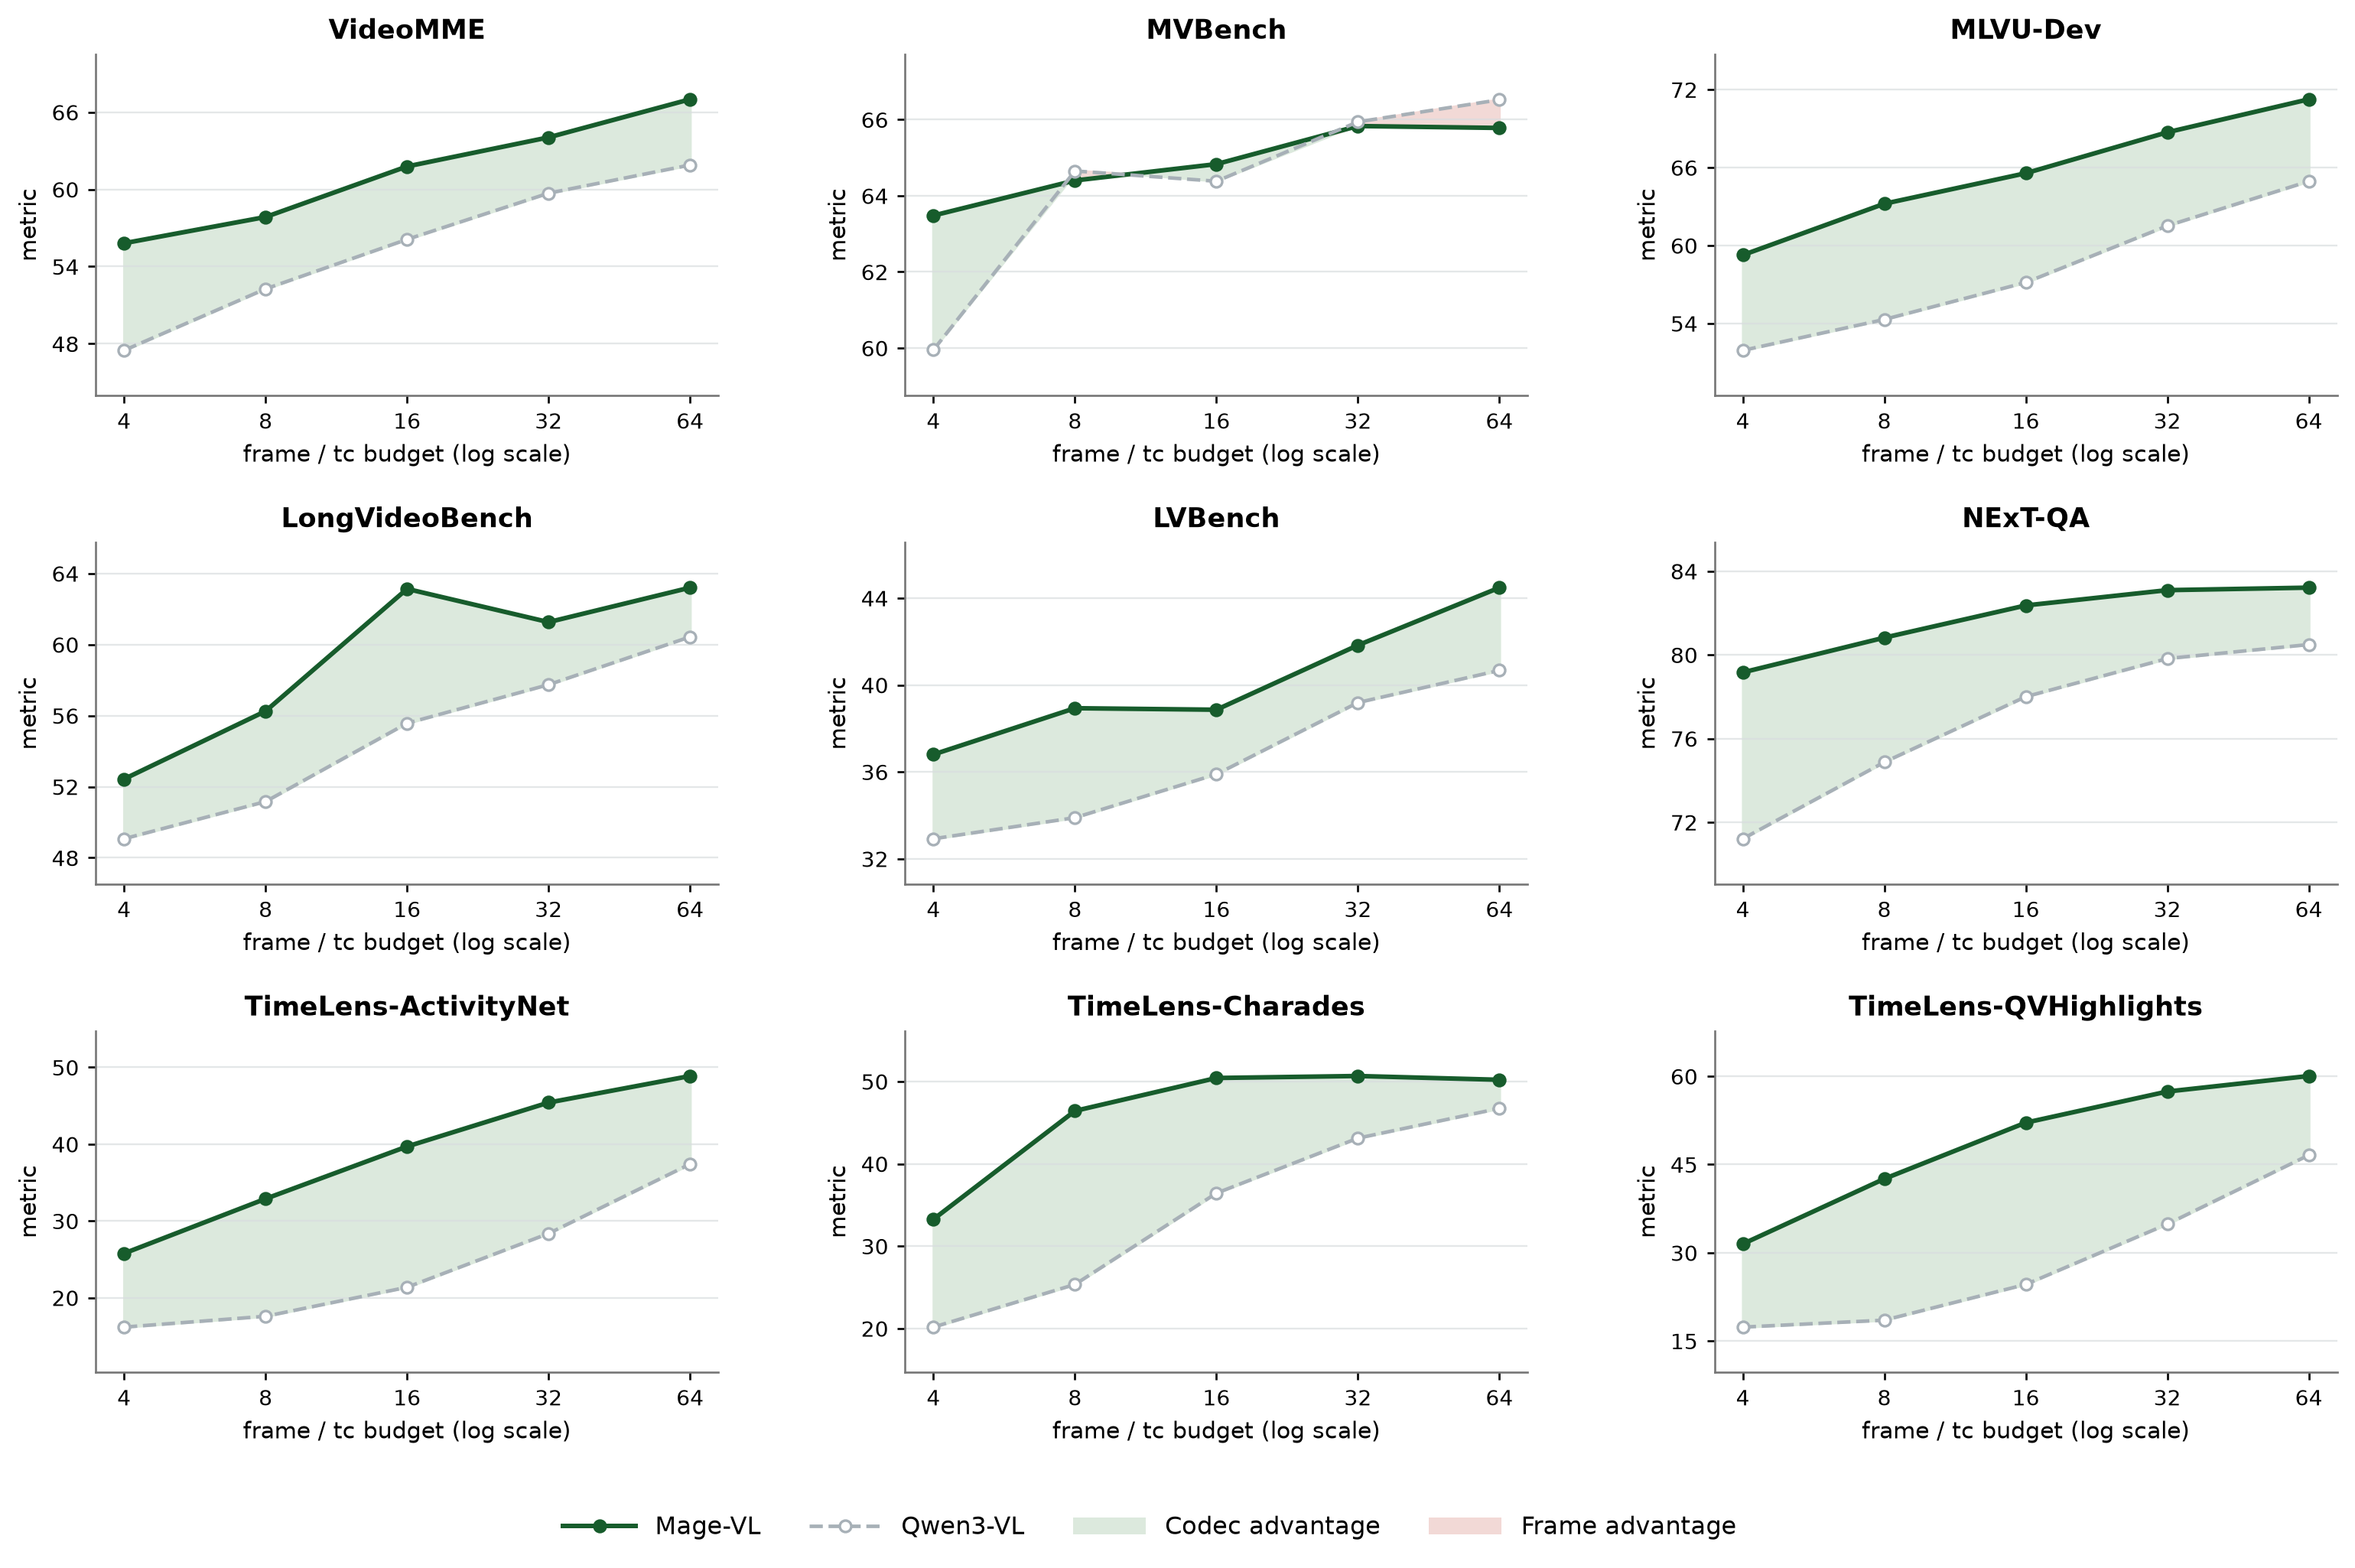
\includegraphics[width=\textwidth]{figures/tc_vs_frame_3x3.png}
  \caption{\textbf{Codec inputs versus uniform frame sampling across input budgets.}
  Frame-$N$ uses $N$ uniformly sampled RGB frames, whereas tc-$N$ targets $N$ codec canvases constructed from $8N$ source frames. Shaded regions highlight the performance gain of codec-native tokenization.}
  \label{fig:tc_vs_frame_scaling}
\end{figure*}


\paragraph{Accuracy-budget scaling.}
As illustrated in Fig.~\ref{fig:tc_vs_frame_scaling}, codec-native tokenization establishes a consistently superior accuracy-efficiency frontier over uniform sampling across long-video and fine-grained temporal tasks. 
Crucially, the performance advantage (\emph{green shaded area}) is most pronounced in low-to-medium budget regimes ($N \le 16$). On dense temporal localization benchmarks such as TimeLens-ActivityNet, TimeLens-Charades, and TimeLens-QVHighlights, sparse uniform sampling frequently misses crucial short-duration events, whereas tc-$N$ retains vital temporal evidence even at $N=4$. 
On long-video QA benchmarks (e.g., VideoMME, LVBench, and MLVU-Dev), tc-$N$ steadily outscales uniform sampling across all budgets ($4 \le N \le 64$). 
The only notable boundary case occurs on MVBench, where both representations converge at high frame budgets, as its short clip structures offer fewer temporally redundant regions for codec compression to exploit. Overall, codec tokenization acts as a dynamic capacity reallocator—pruning temporal redundancies to maximize information density per visual token.



% ------------------ 3. Inference Time & Pareto Frontier (Table 5) ------------------
\paragraph{Pareto efficiency in wall-clock time.}
Table~\ref{tab:understand_video_tc8} further highlights the practical wall-clock inference advantages of \magevl. 
By compressing redundant video content prior to vision encoding, \magevl achieves superior accuracy while drastically reducing latency. For instance, on VideoMME, \magevl under \emph{tc8} achieves $57.9\%$ accuracy in just $270\,\mathrm{s}$ wall-clock time—outperforming Qwen3-VL ($59.7\%$ at $463\,\mathrm{s}$) in compute time while matching its accuracy at \emph{tc16} ($61.8\%$ at $439\,\mathrm{s}$). On NExT-QA~\cite{xiao2021next}, \magevl (\emph{tc8}) cuts the evaluation wall-clock time from $1460\,\mathrm{s}$ down to $415\,\mathrm{s}$ ($3.5\times$ speedup) while achieving higher accuracy ($80.8\%$ vs. $79.8\%$). These results confirm that codec-native visual representation delivers genuine end-to-end inference speedups alongside strong empirical accuracy gains.

\begin{promptbox}
\large
\textbf{\textit{Finding 5:}}
\textbf{Codec-Native Inputs Significantly Boost Video Representation Efficiency.}
By dynamically packing motion-salient patches across extended temporal horizons, codec-native tokenization establishes a superior accuracy-efficiency frontier over uniform frame sampling, achieving substantially higher performance under matched token budgets and up to $3.5\times$ wall-clock inference speedups.
\end{promptbox}






